% Compile with XeLaTeX (needed for Devanagari):
%   xelatex report && bibtex report && xelatex report && xelatex report
\documentclass[11pt]{article}
\usepackage[final]{acl}

\usepackage{fontspec}
\IfFontExistsTF{TeX Gyre Termes}{\setmainfont{TeX Gyre Termes}}{\setmainfont{Times New Roman}}
\IfFontExistsTF{Noto Serif Devanagari}
  {\newfontfamily\devfont[Script=Devanagari,Scale=0.95]{Noto Serif Devanagari}}
  {\IfFontExistsTF{Devanagari MT}
    {\newfontfamily\devfont[Script=Devanagari]{Devanagari MT}}
    {\newfontfamily\devfont[Script=Devanagari]{Kohinoor Devanagari}}}
\newcommand{\hi}[1]{{\devfont #1}}
\newcommand{\slot}[1]{{\normalfont\{#1\}}}  % template slot inside Devanagari text

\usepackage{microtype}
\usepackage{graphicx}
\usepackage{booktabs}
\usepackage{array}
\usepackage{amsmath}
\usepackage{tikz}
\usetikzlibrary{positioning,arrows.meta}

\newcommand{\main}{\hi{मैं}}  % the first-person pronoun of the frame
\newcommand{\aap}{\hi{आप}}
\newcommand{\tum}{\hi{तुम}}

\title{Who Is Speaking, and to Whom? \\
Tracing Speaker Gender, Honorifics and Kinship in Hindi inside Gemma-3}

\author{Aaditya Bhatia \and Aryan Chaudhary \\
  IIIT Hyderabad \\
  \texttt{aaditya.bhatia@research.iiit.ac.in}}

\begin{document}
\maketitle

\begin{abstract}
Hindi makes a model choose between forms that English collapses: the speaker's gender in first-person verbs (\hi{गई}/\hi{गया}), the formality of ``you'' (\aap{}/\tum{}), and the side of the family in kinship terms (\hi{मामा}/\hi{चाचा}). The information is never in the word itself; it has to come from the context. We trace all three in Gemma-3-4B with token-aligned minimal pairs, activation patching, probes, steering and Gemma Scope~2 sparse autoencoders. Speaker gender (96.8\% accuracy) travels name $\to$ \main{} (``I'') $\to$ verb: attention layer 14 copies it onto the pronoun, one SAE feature there fires on every female-speaker prompt and none of the male ones, and head L25H6 carries it to the verb (75\% of the effect). Honorifics (96.4\%) take a parallel route through the opening quote mark, and the same head L25H6 reads them from there, although the features it moves are different. Kinship is not computed at all: accuracy is at chance and the model prefers paternal terms. Each task has a default when the cue is missing (masculine, formal, paternal); late MLPs write almost all of the masculine one but only part of the formal one. Gender errors come from female names that are also nouns (\hi{कविता}, ``poem''): the model's female-name feature never fires on them. Honorific errors keep the cue and are repaired by steering. Code and data: \url{https://github.com/BhatiaAadi/hindi-speaker-gender-interp}.
\end{abstract}

% =====================================================================
\section{Introduction}

English \emph{I went} carries no gender, \emph{you} carries no formality, and \emph{uncle} does not say whose brother he is. Hindi marks all three: a woman says \hi{मैं गई} and a man \hi{मैं गया}; a student asks a teacher \aap{} but a friend \tum{}; the mother's brother is \hi{मामा} and the father's younger brother \hi{चाचा}. LLMs make systematic errors on each of these~\cite{morphogen2026,honorific2025,pardasani2026}, but benchmarks only measure behaviour. We ask \emph{how} a model moves the deciding information from the context to the answer, what it does when there is no cue, and what goes wrong when it fails.

We follow the research questions of our proposal: \textbf{RQ1} behaviour and defaults; \textbf{RQ2} is a correct answer caused by the cue?; \textbf{RQ3} which positions, layers, heads, MLPs and features carry it?; \textbf{RQ4} when the model is wrong, is the cue missing or unused? The hypotheses were
\textbf{H1}: most failures are readout failures (the cue is readable at the answer position but not used), and steering repairs some;
\textbf{H2}: two-step kinship terms compute the intermediate relative in middle layers;
\textbf{H3}: with no cue the model defaults to masculine and paternal forms, written by late MLPs;
\textbf{H4}: a few heads fetch the speaker from the name, like IOI name movers~\cite{wang2022}.
After feedback on scope we made speaker gender the main study and added honorifics and kinship as shorter studies with the same pipeline, in one model (Gemma-3-4B~\cite{gemma3}).

\paragraph{Findings.} (i) Neither cue goes straight to the answer. Speaker gender is first attached to the pronoun \main{}, honorific status to the opening quote mark, and one head, L25H6, reads both from there (Figure~\ref{fig:circuit}). (ii) Single SAE features carry most of the effect at these points. (iii) Kinship side is not computed. (iv) Each task has a default; late MLPs write the masculine one (H3). (v) H1 depends on the task: gender errors lose the cue at the name, honorific errors keep it.

\begin{figure}[t]
\centering
\begin{tikzpicture}[
  tok/.style={draw,rounded corners=2pt,minimum height=0.55cm,inner sep=2pt,font=\footnotesize},
  arr/.style={-{Stealth[length=1.6mm]},thick},
  lab/.style={font=\scriptsize,align=center}]
\node[tok] (n) at (0,0) {\hi{सीमा} (name)};
\node[tok] (p) at (2.75,0) {\main{} (``I'')};
\node[tok] (a) at (5.5,0) {\hi{बाज़ार} $\to$ \hi{गई}};
\draw[arr] (n) -- node[lab,above]{attn L14\\H1, H3} (p);
\draw[arr] (p) -- node[lab,above]{L25H6} (a);
\node[lab,below=0.1cm of n] {layers 0--14};
\node[lab,below=0.1cm of p] {15--25: MLP 18,\\SAE \#7999};
\node[lab,below=0.1cm of a] {26--33; default:\\MLPs 26, 29, 30, 32};
\node[tok] (n2) at (0,-1.9) {\hi{शिक्षक} (addr.)};
\node[tok] (q) at (2.75,-1.9) {\texttt{"} (quote)};
\node[tok] (a2) at (5.5,-1.9) {\hi{"क्या} $\to$ \aap{}};
\draw[arr] (n2) -- node[lab,above]{L13--20\\MLP 20} (q);
\draw[arr] (q) -- node[lab,above]{L25H6\\L26H7} (a2);
\node[lab,below=0.1cm of n2] {layers 0--15};
\node[lab,below=0.1cm of q] {16--25};
\node[lab,below=0.1cm of a2] {26--33:\\SAE \#11554};
\end{tikzpicture}
\caption{How Gemma-3-4B moves speaker gender (top) and the addressee's status (bottom) to the answer, from residual, component, head and SAE-feature patching (\S\ref{sec:route}, \S\ref{sec:sae}).}
\label{fig:circuit}
\end{figure}

% =====================================================================
\section{Related work}

\paragraph{Hindi in LLMs.} MORPHOGEN~\cite{morphogen2026} finds gaps in first-person gender agreement in French, Arabic and Hindi across 15 LLMs; \citet{honorific2025} find that LLMs use Hindi and Bengali honorifics more for men; \citet{pardasani2026} find that models recognise kinship terms far better than they produce them, with a paternal advantage in Hindi. All measure behaviour only.

\paragraph{Circuits and methods.} Subject--verb agreement circuits for person and number have been compared across languages~\cite{ferrando2024,gidi2026}, and Hindi--Urdu agreement has been modelled as a search process~\cite{zhou2024}. Our tasks need the right referent, as in indirect-object identification~\cite{wang2022}; \citet{vig2020} located gender bias with causal mediation. We use activation patching~\cite{meng2022,zhang2024,heimersheim2024}, the logit lens~\cite{nostalgebraist2020}, direct logit attribution (DLA)~\cite{elhage2021}, probes with control tasks~\cite{hewitt2019,belinkov2022}, steering~\cite{turner2023} and sparse autoencoders~\cite{cunningham2024,rajamanoharan2024,gemmascope2}. Lens readings of multilingual models are contested~\cite{wendler2024,bayazit2026,panchal2026}, so every claim rests on an intervention. Late MLPs that promote output tokens~\cite{geva2022} are candidates for writing defaults.

% =====================================================================
\section{Data}
\label{sec:data}

Every prompt ends right before the word the model must choose, and each \emph{clean} prompt has a \emph{corrupt} twin that differs in exactly one token, the cue, which flips the answer. All cues and answers are single tokens (or two-token words whose first token decides), placed mid-sentence; a script checks equal length and the single differing position for every item. Table~\ref{tab:data} summarises the three tasks. Native Hindi speakers (the authors) checked names, frames, templates and samples of every dataset.

\begin{table}[t]
\centering\small
\setlength{\tabcolsep}{3pt}
\begin{tabular}{>{\raggedright\arraybackslash}p{1.35cm}>{\raggedright\arraybackslash}p{3.85cm}r}
\toprule
Task & Example (cue $\to$ swap; answer) & Items \\
\midrule
Speaker gender & \hi{फ़ोन पर सीमा ने कहा, "मैं कल बाज़ार} $\to$ \hi{गई} (\hi{सीमा}$\to$\hi{राहुल}: \hi{गया}) & 3,396 \\
Honorifics & \hi{बाद में नेहा ने अपने शिक्षक से पूछा, "क्या} $\to$ \aap{} (\hi{शिक्षक}$\to$\hi{दोस्त}: \tum{}) & 1,800 \\
Kinship & \hi{हम माँ के छोटे भाई को} $\to$ \hi{मामा} (\hi{माँ}$\to$\hi{पिता}: \hi{चाचा}) & 162 \\
\bottomrule
\end{tabular}
\caption{The three tasks. Items include no-cue prompts.}
\label{tab:data}
\end{table}

\paragraph{Speaker gender.} Twelve frames cover five verb pairs (\hi{गई/गया}, \hi{थी/था}, \hi{रही/रहा}, \hi{जाती/जाता}, \hi{आई/आया}); the ending after the answer (\hi{गई थी}, \hi{रही हूँ}) is not in the prompt. A name of one of 20 female and 20 male names (paired; split 12/4/4 into train/dev/test) is placed by five cue templates: two quotations (T1, T2), an introduction (T3 \hi{नमस्ते, मेरा नाम \slot{N} है।}), a diary (T4 \hi{यह \slot{N} की डायरी है।}) and a letter (T5). This gives 2,400 cue items, 36 no-cue items (\hi{फ़ोन पर उसने कहा, "}\ldots) and 960 distractor items with a second name of the other gender marked by \hi{से}, nearer to the answer than the \hi{ने}-marked speaker (D1) or farther (D2).

\paragraph{Honorifics.} The prompt is a quoted question, \hi{बाद में \slot{S} ने अपने \slot{A} से पूछा, "क्या}, and the answer is the pronoun. Eight addressee pairs of the same gender (so \hi{अपने/अपनी} does not change) contrast a higher-status addressee with a close or younger one: \hi{शिक्षक/दोस्त}, \hi{अध्यापक/मित्र}, \hi{डॉक्टर/बेटे}, \hi{पिताजी/बच्चे}, \hi{सर/यार}, \hi{बॉस/भाई}, \hi{दादी/बेटी}, \hi{टीचर/बहन} (split 5/1/2). Six speakers, six quote openings and three templates, R1 (\hi{पूछा}), R2 (\hi{कहा}) and R3 with the addressee \emph{before} the speaker, give 1,728 items, plus 72 with no addressee.

\paragraph{Kinship.} The parent word is swapped (\hi{माँ/पिता}, \hi{मम्मी/पापा}, \hi{माता/पिता}) for six relations: \hi{छोटे भाई} (\hi{मामा/चाचा}), \hi{पिता} (\hi{नाना/दादा}), \hi{माँ} (\hi{नानी/दादी}), \hi{बहन} (\hi{मौसी/बुआ}) and two two-step relations (\hi{मौसा/फूफा}, \hi{मामी/चाची}), in five prompt types: two definitions, a short story, English (\emph{In Hindi, my mother's younger brother is called}) and a definition preceded by two worked examples. Six prompts give no side (\hi{मेरे अंकल को हिंदी में हम}).

% =====================================================================
\section{Method}
\label{sec:method}

\paragraph{Model and metric.} Gemma-3-4B-pt (34 layers, 8 heads, $d=2560$) in bfloat16 with PyTorch hooks. The metric is the logit difference $\mathrm{LD}=\mathrm{logit}(\text{correct})-\mathrm{logit}(\text{contrast})$ at the last position; accuracy is $\Pr[\mathrm{LD}>0]$, with 95\% intervals from a cluster bootstrap over (template, frame) cells.

\paragraph{Patching.} We keep pairs that the model answers correctly and whose corrupt prompt flips the answer, and patch activations from one run into the other. The effect $(\mathrm{LD}_\text{patched}-\mathrm{LD}_\text{corrupt})/(\mathrm{LD}_\text{clean}-\mathrm{LD}_\text{corrupt})$ is 0 for no change and 1 for full restoration; since every pair occurs in both directions, restoring and replacing give the same pooled number. We patch the residual stream at every layer and position, and attention outputs, MLP outputs and single heads at the answer position and at the token where the residual maps show the cue in the middle layers.

\paragraph{Lens, DLA and probes.} Gemma-3 normalises each sublayer's output before adding it, so the residual is the exact sum of post-norm attention and MLP outputs; freezing the final norm scale makes the LD linear in it (parts sum to the LD within 0.09). Probes are $L_2$ logistic regressions trained on train names (or addressees) and tested on unseen ones, with a control task that gives each name a random fixed label~\cite{hewitt2019}.

\paragraph{Steering.} On wrong items we add $\alpha\lVert\mu_1-\mu_0\rVert$ times a unit direction (difference of means, probe, or 20 random) at the answer position, at $L^\ast$ (best dev probe layer) and at $L_\text{use}$ (first layer where patching the answer position restores half of the effect).

\paragraph{Sparse autoencoders.} We use Gemma Scope~2 JumpReLU SAEs on the residual stream (16k features, $L_0\approx100$--$170$)~\cite{gemmascope2,rajamanoharan2024} at three sites per task: the cue word (layer 9), the middle-layer carrier (\main{}, layer 20; quote mark, layer 22) and the answer position (layer 26). Features are ranked by the class difference of mean activation on training names only. On held-out pairs we patch only the top-$k$ features' change, $\sum_{f\in S}(a^\text{clean}_f-a^\text{corr}_f)\,W_\text{dec}[f]$, into the corrupt run, and compare with $k$ random active features, all features, and the full residual at that site.

% =====================================================================
\section{Results}

\subsection{Behaviour and defaults (RQ1, RQ2, H3)}

\begin{table}[t]
\centering\small
\setlength{\tabcolsep}{4pt}
\begin{tabular}{lccc}
\toprule
 & Gender & Honorifics & Kinship \\
\midrule
Accuracy & 96.8 & 96.4 & 52.6 \\
Flip on cue swap & 96.6 & 96.2 & 7.7$^\dagger$ \\
No-cue default & 83 masc. & 96 \aap{} & 4/6 pat. \\
Errors & 85 & 63 & -- \\
\bottomrule
\end{tabular}
\caption{Behaviour (\%). Flip rate is over correct items; $^\dagger$over all kinship items. 95\% CIs: gender accuracy [94.7, 98.3], honorifics [93.5, 98.7], kinship [48.5, 58.0].}
\label{tab:behaviour}
\end{table}

\paragraph{Gender and honorifics are computed from the cue.} Both reach about 96\% and flip in about 96\% of pairs when the cue is swapped (Table~\ref{tab:behaviour}), so correct answers are caused by the cue (RQ2). A distractor name of the other gender barely matters for gender (D1 98.5\%, D2 100\%), and putting the speaker nearer the answer than the addressee does not confuse honorifics (R3 98.6\%). The answer is often not the top-1 token (62\% and 22\%) because the model may continue with another word (\hi{मैं कल बाज़ार} $\to$ \hi{में}); when it does produce the form, it is right 97.6\% of the time for gender.

\paragraph{Kinship is not computed.} Accuracy is at chance (52.6\%), and swapping \hi{माँ} for \hi{पिता} changes the preferred term in only 7.7\% of items. The LD moves by at most 0.6 logits between the two parents, in every prompt type, including English and two worked examples in the prompt (50\%, no flips). Instead the model has a fixed preference per relation, mostly paternal: \hi{चाची} over \hi{मामी} in 92\% of items, \hi{चाचा} 85\%, \hi{दादा} 81\%, \hi{दादी} 69\%, \hi{बुआ} 62\%; only \hi{मौसा} beats \hi{फूफा} (88\%). Four of the six no-side prompts are paternal (\hi{अंकल} $\to$ \hi{चाचा}, \hi{आंटी} $\to$ \hi{बुआ}). This matches the paternal advantage of \citet{pardasani2026}. Since the side is not used, there is nothing to trace, and we leave kinship (and H2) at behaviour.

\paragraph{Defaults (H3).} With no cue the model prefers the masculine verb in 30 of 36 prompts (LD $-1.04$ [$-1.34$, $-0.76$]) and \aap{} in 69 of 72 (LD $+1.21$). DLA on no-cue prompts attributes the masculine lean to MLPs 26, 29, 30 and 32 ($-0.58$, $-0.43$, $-0.40$, $-0.64$). Zero-ablating them at the answer position takes the masculine share from 83\% to 8\% (LD $+0.94$), while four earlier MLPs (19--22) leave it at 92\% (Table~\ref{tab:default}). MLPs 26, 29 and 30 act for male speakers only ($+1.46$, $+0.64$, $+0.60$ vs.\ $\le 0.24$ for female), so the default is switched off when the speaker is known to be female. The formal default is only partly written by MLPs: zeroing the four that push hardest to \aap{} (32, 19, 17, 25) lowers it from 96\% to 82\% (control 13--16: 100\%). MLP 32 pushes towards both defaults. H3 holds for the masculine default, partly for the formal one, and the paternal default is seen in behaviour.

\begin{table}[t]
\centering\small
\begin{tabular}{lcc}
\toprule
Zeroed MLPs (gender) & LD$_{F-M}$ & \% masc. \\
\midrule
none & $-1.04$ & 83 \\
32 & $-0.54$ & 69 \\
26, 29, 30 & $+0.02$ & 47 \\
26, 29, 30, 32 & $+0.94$ & 8 \\
control: 19--22 & $-1.32$ & 92 \\
\bottomrule
\end{tabular}
\caption{The masculine default on the 36 no-cue prompts after zero-ablating MLPs at the answer position.}
\label{tab:default}
\end{table}

\subsection{The route of the cue (RQ3, H4)}
\label{sec:route}

\begin{figure}[t]
  \centering
  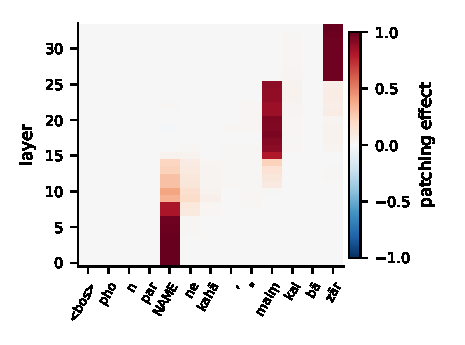
\includegraphics[width=\columnwidth]{figures/resid_map_T1_f01_denoise.pdf}\\[-2pt]
  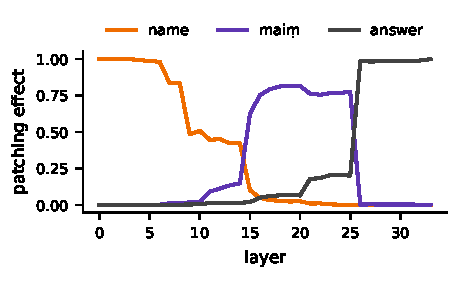
\includegraphics[width=\columnwidth]{figures/resid_positions.pdf}
  \caption{Speaker gender. Top: patching the residual stream at each layer and position for T1 \hi{फ़ोन पर \slot{N} ने कहा, "मैं कल बाज़ार} (38 pairs). Bottom: the name, \main{} and answer positions, averaged over 20 template--frame cells.}
  \label{fig:resid}
\end{figure}

\paragraph{Speaker gender: name $\to$ \main{} $\to$ answer.} Up to layer 8 the whole effect is at the name (Figure~\ref{fig:resid}). At layer 15 it moves onto the frame's pronoun \main{} (0.62; 0.75--0.81 at layers 16--25), and from layer 26 the answer position carries it alone (0.98); before layer 26, patching the answer position restores at most 0.20. All 20 mapped cells, in every template, show this route. Patching components at \main{} (Figure~\ref{fig:components}, right) points to attention layer 14 (0.36), mostly heads L14H1 (0.20) and L14H3 (0.17), then MLP 18 (0.76) and MLP 23 (0.23). From \main{}, L14H3 attends to the speaker's name and picks the \hi{ने}-marked speaker over a distractor both when the distractor is nearer (0.29 vs.\ 0.04) and when it is farther (0.50 vs.\ 0.02); patching at \main{} on distractor items finds the same components. At the answer position a single head dominates: L25H6 restores 0.75 (0.71--0.78 per template), with a direct effect of $+0.82$ logits. It attends to \main{} (0.69) and not to the name (0.005). MLPs 26 (0.37), 23 and 25 (0.21) amplify the signal. The logit lens agrees: the LD reaches its final value between layers 24 and 27. H4 holds in a revised form: speaker heads exist and select the speaker by role, but they write into the pronoun, and a separate head moves the gender to the verb.

\begin{figure}[t]
  \centering
  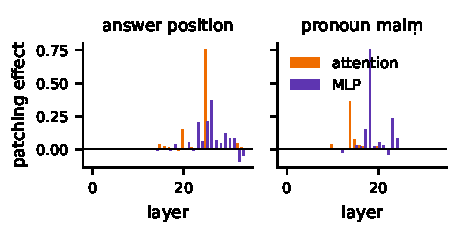
\includegraphics[width=\columnwidth]{figures/attn_mlp.pdf}\\[-2pt]
  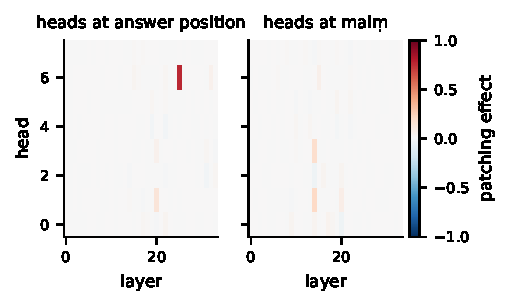
\includegraphics[width=\columnwidth]{figures/heads.pdf}
  \caption{Speaker gender: patching attention and MLP outputs (top) and single heads (bottom), at the answer position and at \main{}.}
  \label{fig:components}
\end{figure}

\begin{figure}[t]
  \centering
  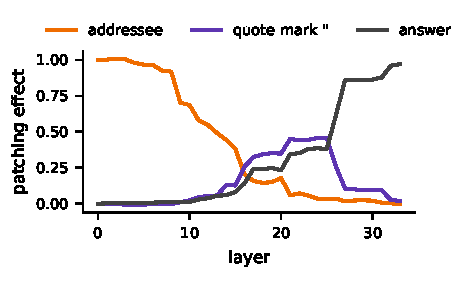
\includegraphics[width=\columnwidth]{figures/honorific/resid_positions.pdf}\\[-2pt]
  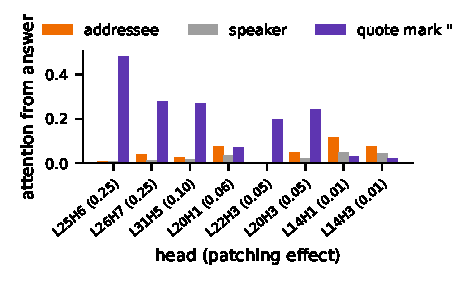
\includegraphics[width=\columnwidth]{figures/honorific/honor_attention.pdf}
  \caption{Honorifics. Top: patching the residual stream at the addressee, the opening quote mark and the answer position (12 cells). Bottom: attention from the answer position of the top heads (patching effect in brackets) and of the gender heads L14H1, L14H3, averaged over R1--R3.}
  \label{fig:honor}
\end{figure}

\paragraph{Honorifics: addressee $\to$ quote mark $\to$ answer.} The addressee carries the effect up to layer 8 ($\ge 0.92$), then hands it on (Figure~\ref{fig:honor}): \hi{से} after it holds 0.16--0.21 at layers 9--15, and the opening quote mark \texttt{"} holds 0.26 at layer 16, 0.33--0.35 at 17--20 and 0.44--0.46 at 21--25. The answer position takes over at layer 26 (0.62; 0.86 at 27). Patching at the quote mark shows several mid-layer writers rather than one: attention layers 20 (0.15), 15 (0.13) and 16 (0.10), MLP 20 (0.23), and heads L20H1 (0.10), L15H6 (0.09) and L13H5 (0.07). At the answer position the top heads are \textbf{L25H6} (0.25) and L26H7 (0.25), stable across R1--R3, with MLP 26 (0.34). L25H6, the gender head, puts 0.48 of its attention on the quote mark in every word order and less than 0.02 on the addressee, the speaker or \hi{से}. The gender copying heads L14H1/L14H3 attend to the addressee but have no effect (0.01). Like \main{} for gender, the token that opens the clause holds the cue in the middle layers, and the same head reads it from there.

\subsection{SAE features (RQ3)}
\label{sec:sae}

\begin{table*}[t]
\centering\small
\setlength{\tabcolsep}{4.2pt}
\begin{tabular}{llcccccccc}
\toprule
Task & Site (layer) & Top feat. & Fires (cl.\ 1 / 0) & top-1 & top-5 & top-20 & rand.-20 & all SAE & full resid. \\
\midrule
Gender & name (9) & \#6249 & 97\% / 0\% & 0.07 & 0.14 & 0.31 & 0.00 & 0.45 & 0.52 \\
 & \main{} (20) & \#7999 & 100\% / 0\% & \textbf{0.48} & 0.50 & 0.51 & 0.00 & 0.51 & 0.68 \\
 & answer (26) & \#12128 & 100\% / 0\% & 0.38 & \textbf{0.91} & 0.93 & 0.00 & 0.95 & 0.98 \\
Honorifics & addressee (9) & \#298 & 100\% / 100\% & 0.01 & 0.01 & 0.06 & 0.01 & 0.61 & 0.74 \\
 & quote mark (22) & \#4438 & 98\% / 100\% & 0.02 & 0.08 & 0.13 & 0.01 & 0.29 & 0.44 \\
 & answer (26) & \#11554 & 74\% / 100\% & \textbf{0.70} & 0.68 & 0.68 & 0.01 & 0.74 & 0.83 \\
\bottomrule
\end{tabular}
\caption{Patching SAE features on held-out pairs (910 gender, 358 honorific): normalised effect of restoring only the top-$k$ features (ranked on training names), $k$ random active features (mean of 10 draws), all features, or the full residual stream at the site. Class 1 is female speaker or formal addressee.}
\label{tab:sae}
\end{table*}

Reconstructing a site with its SAE keeps 81--102\% of the LD (accuracy 94--96\%; 74\% at the honorific answer position, where many items are near the boundary). Table~\ref{tab:sae} shows how much of the cue single features carry.

\paragraph{Gender is carried by a few clean features.} At \main{}, feature \#7999 fires on every female-speaker prompt and on no male one (held-out AUC 1.00), and patching it alone restores 0.48, almost all of what the SAE captures there (0.51); zeroing it in clean runs flips about a third of female-speaker items. At the answer position, five features restore 0.91 of 0.98, and zeroing them brings accuracy to 51\%. At the name the cue is more spread out (top-20: 0.31 of 0.52), but its top feature \#6249 is a female-name feature: it fires on 97\% of female names, never on male ones, and its decoder promotes tokens such as \emph{Kumari}, \emph{Elizabeth} and Gujarati \emph{hatī} (feminine ``was''); \#7746 at \main{} promotes \emph{woman/women}. Random features of the same number restore nothing.

\paragraph{Honorific status is spread out until the answer.} At the addressee and the quote mark, even 20 features restore little (0.06, 0.13) of what all features do, as expected for eight different addressee words. The quote-mark features are still readable: \emph{you/your} and imperatives (\emph{come, join}) favour \tum{}, while a plural-address feature (\emph{folks, guys, ladies}; 81\% vs.\ 2\%) favours \aap{}, which is grammatically plural. At the answer position one feature, \#11554, restores 0.70 of 0.83; its decoder promotes \emph{ты, тебе, thou}, the familiar \emph{you} of other languages, and zeroing it brings accuracy to 50\%.

\paragraph{One head, different features.} The top-20 answer-position features of the two tasks share only two, which fire on most items of both classes and barely separate them (AUC 0.52--0.57), and the decoder directions of the top five differ (cosine $\le0.11$ apart from the shared feature). L25H6 thus moves different features in the two tasks: it is a general mover from the clause-opening token, not a gender head.

\subsection{Failures and repair (RQ4, H1)}
\label{sec:failures}

\paragraph{Gender: noun-like names.} Of the 85 gender errors, 46 are diary items (T4) with \hi{कविता}, \hi{रेखा}, \hi{सीमा} and \hi{पूजा}, which are also nouns (poem, line, border, worship). The model gets 2 of these 48 items right (mean LD $-1.64$, close to the no-cue default) but 98--100\% of the same names in other templates; \hi{यह कविता} alone means ``this poem''. The SAE shows where the cue is lost: the female-name feature \#6249 fires on 99\% of correct female items, on 62\% of these names in other templates, and on \emph{none} of the 47 wrong items; \#7999 at \main{} fires on 2\% of them. The model reads the word as a noun from the start. Probes trained without these names' pairs still read ``female'' at the name position but ``male'' at the answer position from layer 26 (98--100\%), so the information a probe finds at the name is the identity of the word, not the model's female-person feature. These are not readout failures, and H1 is not supported for gender.

\begin{figure}[t]
  \centering
  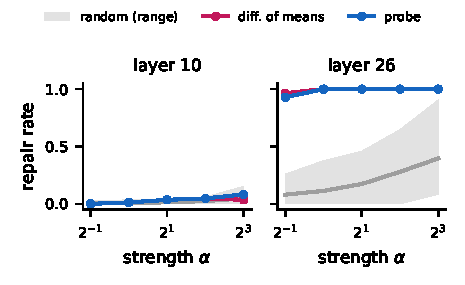
\includegraphics[width=\columnwidth]{figures/steering.pdf}
  \caption{Share of the 85 gender errors repaired by steering at the answer position, at $L^\ast{=}10$ and at $L_\text{use}{=}26$.}
  \label{fig:steering}
\end{figure}

\paragraph{Honorifics: readout failures.} The 63 honorific errors are mostly familiar addressees answered with \aap{} (41: \hi{बच्चे}, \hi{बहन}, \hi{भाई}, \hi{बेटे}, \hi{बेटी}), in line with the formal default. Probes read the addressee's class on all 63 at layers 11 and 26 (held-out addressees; the control task is also high with only eight addressee pairs, so this shows presence, not a clean code). The cue is there but not used: H1 holds for honorifics.

\paragraph{Repair.} Steering at $L_\text{use}=26$ repairs both kinds of error (Figure~\ref{fig:steering}). For gender, the difference-of-means direction repairs 96\% at $\alpha=0.5$ and 100\% from $\alpha=1$, against 8--11\% for random directions on average, without breaking right items. For honorifics it repairs 90\% at $\alpha=0.5$ and 98--100\% from $\alpha=1$ (probe direction 100\%), against 28--38\% for random directions on average; the best random direction also reaches 90\%, because many wrong items are close to the boundary. At $L^\ast$, the first layer with the best probe accuracy (10 and 11), steering is no better than random in either task: probe accuracy picks a layer the model does not use for the decision.

% =====================================================================
\section{Discussion}

\paragraph{A shared reader, task-specific carriers.} In both tasks that the model computes, the cue is not fetched from its source when the answer is written. It is first attached to the token that opens the clause, the subject pronoun \main{} or the opening quote mark, and head L25H6 reads it from there. For gender this mirrors the grammar: the verb agrees with its subject, and the model attaches the speaker's gender to that subject. The carried information is task-specific (different SAE features), while the reader is shared, which suggests a general ``read the clause's context'' head rather than a gender circuit.

\paragraph{Hypotheses.} H1 depends on the task: gender errors lose the cue at the name, because the model does not see a person there; honorific errors keep it and are readout failures. H2 could not be tested, since the model does not compute kinship side at all. H3 is supported for the masculine default (late MLPs, switched off for female speakers), partly for the formal default, and behaviourally for the paternal one. H4 holds in a revised form: the heads that pick the speaker select the \hi{ने}-marked subject over a nearer name, but write into \main{}. Linear readability was a poor guide throughout: the cue is readable at the answer position from about layer 7--11, but used only from layer 26.

\paragraph{Scope.} Compared with the proposal we dropped the Sarvam-1 comparison and the test of H2, and treat kinship at the level of behaviour.

% =====================================================================
\section*{Limitations}

We study one pretrained model on short templated prompts; in real text, speakers and addressees are introduced in many other ways. Hindi verbs have two gender forms, so our gender data is binary; the masculine default we find is itself a problem for speakers whose gender is unknown or non-binary. The noun-like name finding comes from error analysis and rests on four names. Honorific status is reduced to two classes of eight addressees, and familiarity norms differ between families and regions (we kept only items both authors agreed on). Kinship has 156 cue items and no mechanism to trace. Zero-ablation is off-distribution; mean-ablation gave a weaker masculine effect. SAE features are labelled from their top output tokens, which is suggestive only; the 16k SAEs lose part of the effect at some sites (``all SAE'' vs.\ ``full'' in Table~\ref{tab:sae}).

\section*{Ethics statement}

The defaults we localise are biases: an unnamed speaker is treated as male, and kinship terms default to the father's side. All names are common first names, not real people. We used AI assistants for coding and writing support.

\bibliography{references}

\end{document}
